\documentclass[journal]{vgtc}                % final (journal style)
%\documentclass[review,journal]{vgtc}          % review (journal style)
%\documentclass[widereview]{vgtc}             % wide-spaced review
%\documentclass[preprint,journal]{vgtc}       % preprint (journal style)
%\documentclass[electronic,journal]{vgtc}     % electronic version, journal
\let\ifpdf\relax

%% Uncomment one of the lines above depending on where your paper is
%% in the conference process. ``review'' and ``widereview'' are for review
%% submission, ``preprint'' is for pre-publication, and the final version
%% doesn't use a specific qualifier. Further, ``electronic'' includes
%% hyperreferences for more convenient online viewing.

%% Please use one of the ``review'' options in combination with the
%% assigned online id (see below) ONLY if your paper uses a double blind
%% review process. Some conferences, like IEEE Vis and InfoVis, have NOT
%% in the past.

%% Please note that the use of figures other than the optional teaser is not permitted on the first page
%% of the journal version.  Figures should begin on the second page and be
%% in CMYK or Grey scale format, otherwise, colour shifting may occur
%% during the printing process.  Papers submitted with figures other than the optional teaser on the
%% first page will be refused.

%% These three lines bring in essential packages: ``mathptmx'' for Type 1
%% typefaces, ``graphicx'' for inclusion of EPS figures. and ``times''
%% for proper handling of the times font family.

% Math-mode symbol & verbatim
\def\W#1#2{$#1{#2}$ &\tt\string#1\string{#2\string}}
\def\X#1{$#1$ &\tt\string#1}
\def\Y#1{$\big#1$ &\tt\string#1}
\def\Z#1{\tt\string#1}

\usepackage{mathptmx}
%%\usepackage{psfrag}
\usepackage{graphicx}
\usepackage{times}
\usepackage{epstopdf}

\usepackage{amssymb,amsmath,amsthm}
\usepackage[lined,linesnumbered]{algorithm2e}
\usepackage{caption}
\usepackage{subcaption}
\usepackage{multirow}
\usepackage{framed}
\usepackage{tikz}
\usepackage{array}

%% We encourage the use of mathptmx for consistent usage of times font
%% throughout the proceedings. However, if you encounter conflicts
%% with other math-related packages, you may want to disable it.

%% This turns references into clickable hyperlinks.
\usepackage[bookmarks,backref=true,linkcolor=black]{hyperref} %,colorlinks
\hypersetup{
  pdfauthor = {},
  pdftitle = {},
  pdfsubject = {},
  pdfkeywords = {},
  colorlinks=true,
  linkcolor= black,
  citecolor= black,
  pageanchor=true,
  urlcolor = black,
  plainpages = false,
  linktocpage
}

%% If you are submitting a paper to a conference for review with a double
%% blind reviewing process, please replace the value ``0'' below with your
%% OnlineID. Otherwise, you may safely leave it at ``0''.
\onlineid{0}

%% declare the category of your paper, only shown in review mode
\vgtccategory{Technique}

%% allow for this line if you want the electronic option to work properly
\vgtcinsertpkg

%% In preprint mode you may define your own headline.
%\preprinttext{To appear in an IEEE VGTC sponsored conference.}


%%%%%%%%%%%%%%%%%%%%%%%%%%%%%%%%%%%%%%%%%%%%%%%%%%%%%%%%%%%%%%%%%%%%%%%%%%%%%
%
% Math commands
%
%%%%%%%%%%%%%%%%%%%%%%%%%%%%%%%%%%%%%%%%%%%%%%%%%%%%%%%%%%%%%%%%%%%%%%%%%%%%%

\newcommand {\emath}[1]  {\ensuremath{#1}}
\newcommand {\R}         {\emath{\mathbb{R}}}        % Real space
\newcommand {\Real}[1]   {\emath{\mathbb{R}^{#1}}}   % Real space
\newcommand {\Rd}        {\Real{d}}                  % R^d
\newcommand {\Rdone}     {\Real{d+1}}                % R^d+1
\newcommand {\Rk}        {\Real{k}}                  % R^k
\newcommand {\Rtwo}      {\Real{2}}                  % R^2
\newcommand {\Rthree}    {\Real{3}}                  % R^3
\newcommand {\Rfour}     {\Real{4}}                  % R^4
\newcommand {\Sphere}[1] {\emath{\mathbb{S}^{#1}}}   % Sphere
\newcommand {\Sk}        {\Sphere{k}}                % S^k
\newcommand {\Sd}        {\Sphere{d}}                % S^d
\newcommand {\BB}        {\emath{\mathbb{B}}}        % B
\newcommand {\Ball}[1]   {\emath{\mathbb{B}^{#1}}}   % B^{#1}
\newcommand {\Ballep}    {\emath{B^{\epsilon}_{p}}}  % B^e_p
\newcommand {\cl}        {\emath{\mathrm{cl}}}       % cl
\newcommand {\cb}        {\emath{\mathbf{c}}}        % bold c
\newcommand {\eb}        {\emath{\mathbf{c}}}        % bold e
\newcommand {\tpi}       {\emath{\tilde{\pi}}}       % \pi~
\newcommand {\gDim}[1]   {\emath{#1 \times #1 \times #1}} % DxDxD

\newcommand {\tg}        {\emath{\tilde{g}}}
\newcommand {\tn}        {\emath{\tilde{n}}}
\newcommand {\IV}        {\emath{\mathcal{I_V}}}
\newcommand {\Orth}      {\emath{\mathcal{O}}}
\newcommand {\hN}        {\emath{\widehat{N}}}
\newcommand {\XX}        {\emath{\mathcal{X}}}

\newtheorem{proposition}{Proposition}
\newtheorem{corollary}{Corollary}[proposition]
\newtheorem{lemma}[proposition]{Lemma}


%%%%%%%%%%%%%%%%%%%%%%%%%%%%%%%%%%%%%%%%%%%%%%%%%%%%%%%%%%%%%%%%%%%%%%%%%%%%%
%
% tikz block styles
%
%%%%%%%%%%%%%%%%%%%%%%%%%%%%%%%%%%%%%%%%%%%%%%%%%%%%%%%%%%%%%%%%%%%%%%%%%%%%%

\usetikzlibrary{shapes,arrows}

\tikzstyle{action} = [rectangle, draw, text centered, node distance=4cm, minimum height=4em]
\tikzstyle{source} = [draw, ellipse, text centered, node distance=1.5cm, minimum height=4em, text width=3cm]
\tikzstyle{sink} = [draw, ellipse, text centered, node distance=2cm, minimum height=4em]
\tikzstyle{line} = [draw, -latex']
\tikzstyle{figlabel} = [text centered, node distance=1.5cm, text width=1cm]

%%%%%%%%%%%%%%%%%%%%%%%%%%%%%%%%%%%%%%%%%%%%%%%%%%%%%%%%%%%%%%%%%%%%%%%%%%%%%
%
% algorithm2e keywords and commands
%
%%%%%%%%%%%%%%%%%%%%%%%%%%%%%%%%%%%%%%%%%%%%%%%%%%%%%%%%%%%%%%%%%%%%%%%%%%%%%

% algorithm2e global keywords
\SetKw{Function}{Function}
\SetKw{true}{true}
\SetKw{false}{false}
\SetKw{KwAnd}{and}
\SetKw{KwOr}{or}
\SetKw{true}{true}
\SetKw{false}{false}
\SetKw{KwElse}{else}
\SetKw{KwDownTo}{downto}
\SetKwData{NULL}{NULL}
\SetKwInOut{Input}{Input}
\SetKwInOut{Output}{Output}
\SetKwInOut{Result}{Result}
\SetKwInOut{Requires}{Requires}
\ResetInOut{Requires1}
\SetKwComment{NoLineNum}{}{}
\SetCommentSty{textit}
\SetArgSty{textrm}
\SetFuncSty{textsc}
\SetAlgoLined

\IncMargin{1ex}

\SetKwFunction{AngleTest}{AngleTest}
\SetKwFunction{ScalarTest}{ScalarTest}
\SetKwFunction{ReliableGrad}{ReliableGrad}
\SetKwFunction{MergeSharp}{MergeSharp}
\SetKwFunction{FindSharp}{FindSharp}
\SetKwFunction{CountDegree}{CountDegree}
\SetKwFunction{SelectiveFindSharp}{SelectiveFindSharp}
\SetKwFunction{Magnitude}{Magnitude}
\SetKwFunction{Angle}{Angle}
\SetKwFunction{Distance}{Distance}
\SetKwData{Grid}{Grid}
\SetKwData{numAgree}{numAgree}
\SetKwData{errorDist}{errorDist}
\SetKwData{maxErrorDist}{maxErrorDist}
\SetKwData{numIter}{numIter}

% Algorithm function names and variables
\SetKwFunction{DoesOrthMatch}{DoesOrthMatch}
\SetKwFunction{DoesOrthMatchA}{DoesOrthMatchA}
\SetKwFunction{DoesOrthMatchB}{DoesOrthMatchB}
\SetKwFunction{ExtendReliable}{ExtendReliable}


\SetKwData{Center}{Center}
\SetKwData{Centroid}{Centroid}
\SetKwData{isovLoc}{isovLoc}
\SetKwData{numLargeEigenvalues}{numLargeEigenvalues}

% algorithm2e reset line number
\newcommand {\ResetAlgoLineNumber} {\setcounter{AlgoLine}{0}}

\SetAlgoCaptionSeparator{.}




\title{Visualizing flow fields using fractal dimensions}

%% This is how authors are specified in the journal style

%% indicate IEEE Member or Student Member in form indicated below
\author{Ross Vasko, Han-Wei Shen and Rephael Wenger}
\authorfooter{
The Ohio State University. E-mail: vasko.38@osu.edu, shen.94@osu.edu
 and wenger.4@osu.edu}



\abstract{
Streamlines are a popular way of visualizing flow in vector fields.
A major challenge in streamline visualization is selecting the streamlines
for visualization.
Rendering too many streamlines clutters the visualization and makes
features of the field difficult to identify. 
Rending too few streamlines causes viewers to completely miss features
of the flow field not rendered. 

The fractal dimension of a streamline represents its space-filling properties.
To identify complex or interesting streamlines, 
we build a regular grid of scalar values 
which represent the fractal dimension of streamlines around each grid vertex.
High fractal dimension indicates vortices or turbulent regions.
We use this scalar grid both to filter streamlines by fractal dimension
and to identify and visualize regions containing vortices and turbulence.
We describe an interactive tool which allows for quick streamline selection
and visualization of regions containing vortices and turbulence.
}

%% Keywords that describe your work. Will show as 'Index Terms' in journal
%% please capitalize first letter and insert punctuation after last keyword
\keywords{Streamlines, fractal dimension.}

%% ACM Computing Classification System (CCS). 
%% See <http://www.acm.org/class/1998/> for details.
%% The ``\CCScat'' command takes four arguments.

\CCScatlist{ % not used in journal version
\CCScat{I.3.5}{Computer Graphics}{Computational Geometry and Object Modeling}
}

%% Uncomment below to include a teaser figure.
%\teaser{
%}

%% Uncomment below to disable the manuscript note
%\renewcommand{\manuscriptnotetxt}{}

%% Copyright space is enabled by default as required by guidelines.
%% It is disabled by the 'review' option or via the following command:
% \nocopyrightspace

\renewcommand{\textfraction}{0.2}
\renewcommand{\dbltopfraction}{0.8}	
\renewcommand{\topfraction}{0.8}	


%%%%%%%%%%%%%%%%%%%%%%%%%%%%%%%%%%%%%%%%%%%%%%%%%%%%%%%%%%%%%%%%
%%%%%%%%%%%%%%%%%%%%%% START OF THE PAPER %%%%%%%%%%%%%%%%%%%%%%
%%%%%%%%%%%%%%%%%%%%%%%%%%%%%%%%%%%%%%%%%%%%%%%%%%%%%%%%%%%%%%%%%

\begin{document}

\maketitle

\section{Introduction}

A vector field in 3D is a function $f: \Rthree \Rightarrow \Rthree$.
A flow field is a specific type of vector field that represents the flow of some fluid.
Each point in a 3D flow field represents a velocity vector of the fluid.
Flow fields are used in several different fields of science and engineering.
They can be used to represent storms, air flow during wind tunnel tests, or blood flow.
Effectively visualizing flow fields are crucial to their interpretation.
An ideal visualization will communicate the structure and physics of the flow field.
Unfortunately, identifying meaningful and interesting structures is often computationally difficult due to the size of the flow field data sets.

A common way to visualize flow fields is with streamlines.
A streamline is a curve that is tangent to the velocity vector of the flow field at each point of the curve.
Streamlines are computationally inexpensive to generate and allow a viewer to see the behavior of a region of the flow field.
But, a large challenge in using streamlines to visualize flow fields is choosing which streamlines to display.
If too many streamlines are displayed, the visualization quickly becomes cluttered and interesting features or behavior of the flow field become hard to identify.
If an arbitrary sampling is chosen to display less streamlines, some interesting features of the flow field could potentially not be displayed at all.

To address this challenge, we look for a way to identify interesting or complex streamlines or regions of the flow field.
The box-counting dimension measures how a densely a set fills a metric space.
The box counting dimension of a set S is defined as:
\begin{equation} dim(S) = \lim_{\epsilon \to 0}  \frac{\log N(\epsilon)}{\log(\epsilon^{-1})}\end{equation}
Where $N(\epsilon)$ is the minimum number of boxes needed to cover the set.
Using a previously proposed modified definition of the box counting dimensions, we will measure how streamlines fill a space to determine their complexity.

Once we have these complexity measurements of streamlines around the flow field, we build a scalar field of complexity values.
This scalar field allows us to easily identify which regions of the flow field are complex.
Also, using this scalar field, we can apply a variety of visualization techniques to allow the user different insight on the data.

\section{Related Work}

In a previous work by Chaudhuri, he introduces measuring the streamline complexity with fractal dimensions to oberserve behavior at different scales.
The motivation for moving to such a measurement was to focus solely on the geometry of the line and to prevent limiting oneself to only searching for some certain fluid property.
By setting parameters in the box counting ratio, the fractal dimension measurements are used in this work to be able to the identify streamline features at different scales.
Features in the flow field can then be organized by their complexity as well as what scale the feature appears in.

\section{Box Counting Ratio}

The box counting ratio does not calculate an integer dimension for a set.
Rather, depending on how the set fills a space, the dimension is some real number between 0 and 3 for a space filling fractal in 3D.
But, because our streamlines generated from a simulation are simply a series of connected straight line segments, this strict definition would meausre each streamline as having a fractal dimension as 1.
Regardless, calculating this limit exactly becomes infeasible to do on a computer for each streamline.
Instead, we use an alternative definition that allows us to simply approximate the box counting ratio.

Khoury and Wenger defined a box counting ratio approximation in a previous work on examing the properties of isosurfaces using fractal dimensions.
The idea of this new approximation is to sample an object at two different resolutions and then estimate the box counting ratio using these two measurements.
The new approximated box counting ratio of a set S is defined as:
\begin{equation} dim_{approx}(S) = \log_2\frac{N(\frac{\epsilon}{2})}{N(\epsilon)}\end{equation}
where $N(\epsilon)$ in this case is simply the number of boxes that the set will intersect on a fixed grid.

We then measure the fractal dimension of the streamlines by defining a fixed grid, counting the number of boxes that the streamlines intersects at the resolution of $\frac{\epsilon}{2}$ and ${\epsilon}$, and then solving for the final box counting dimension.
With this new formula, we expect that the straight and simple streamlines will have a fractal dimension near 1, as they do not have any space filling properties.
As the streamline becomes more complex and fills a 3D region more densely, we expect the fractal dimension to increase exceed 2.
These measurements are illustrated in Fig. \ref{fig:box_counting_calcs}

\begin{figure}[t]
	\centering
		\begin{minipage}{0.47\linewidth}
			\centering \small
			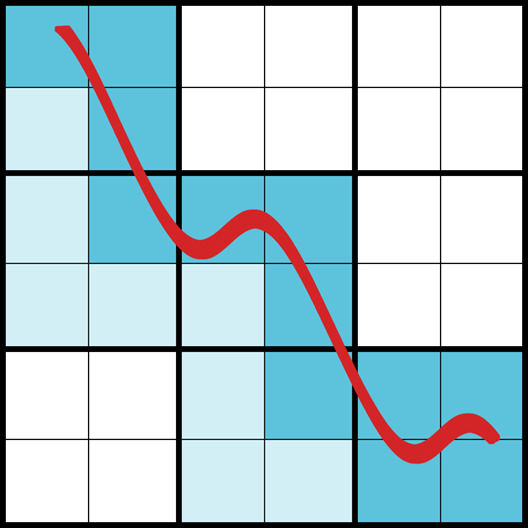
\includegraphics[height = 0.7\linewidth]{line.png}\\(a) simple line with box counting ratio of $\log_2\frac{12}{5} = 1.26$\vspace{0.2em}
		\end{minipage}
		\begin{minipage}{0.47\linewidth}
			\centering \small
			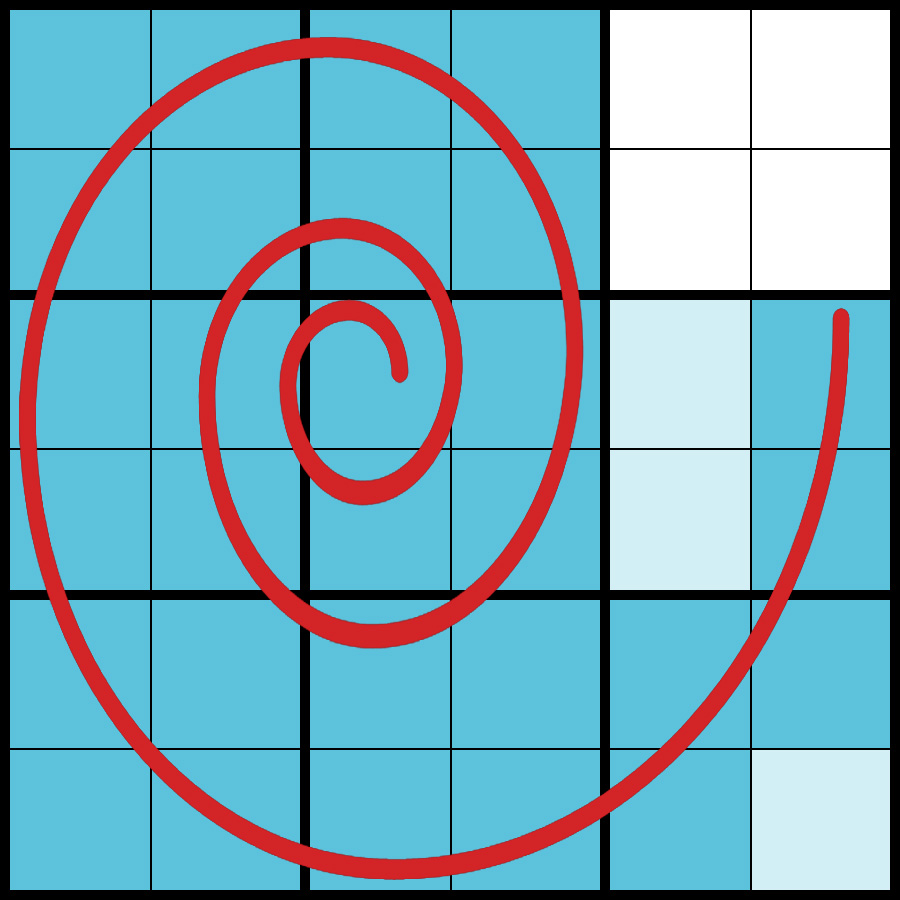
\includegraphics[height = 0.7\linewidth]{spiral.jpg}\\(b) complex line with box counting ratio of $\log_2\frac{29}{8} = 1.86$\vspace{0.2em}
		\end{minipage}
	\caption{Example of box counting ratio calculations on streamlines.}
	\label{fig:box_counting_calcs}
\end{figure}

\section{Streamline Complexity Grid}

For each regular point $p$ in a vector field $f: \Rthree \Rightarrow \Rthree$,
let $\zeta_p$ be the unique streamline passing through $p$.
Define $\phi_w(p)$ as the local box counting ratio of $\zeta_p$
in a $\gDim{w}$ region around $p$,
where boxes have edge lengths 1 and 2.
Function $\phi_w$ defines a scalar field on the regular points of $f$.
The scalar $\phi_w(p)$ represents the complexity of a streamline through $p$ in a $\gDim{w}$ neighborhood of $p$.
We call the scalar field $\phi_w$, the streamline complexity field of $f$.

To compute the set of streamlines, we first seed a streamline from each regular point voxel $v$ in our vector field $f$.
We then calculate the box counting dimensions of each of these streamlines using the previously described box counting dimension algorithm.
If the streamline intersects more than a predefined cutoff of $c_s$ boxes of edge length 2, then the streamline is stored.
If the streamline does not intersect more than $c_s$ boxes, it is discarded.

To compute the local box counting ratio of $\zeta_v$ in a $\gDim{w}$ region centered at $v$, we take a subset of the streamline, $\zeta_s$, that precisely includes the portion of $\zeta_v$ that is within the $\gDim{w}$ region.
The box counting dimension of $\zeta_s$ is then computed using the previously described box counting dimension algorithm.
Similarly to the streamline generation step, it is also ensured that $\zeta_s$ more than $c_v$ boxes of edge length 2.
If $\zeta_s$ does meet the cutoff requirement, the box counting dimension is considered a value estimate, if not, the value is discarded.

To construct a scalar grid representing the streamline complex field of $f$, a set of streamlines are generated as previously described.
For each streamline $\zeta_v$ that intersects voxel $v$, we compute the local box counting dimension of $\zeta_v$.
If $\zeta_v$ meets the cutoff requirement, the resulting box counting dimension is stored in a list with all other box counting dimensions calculated for $v$.
Once the local box counting dimension of all of the streamlines that intersect $v$ have been calculated, we take the $P$\textsuperscript{th} percentile of the local box counting dimension list and store this value as $v$'s complexity value.
Let the streamline whose local box counting dimension was measured as the $P$\textsuperscript{th} percentile local box counting dimension for voxel $v$ be denoted as $v_\zeta$.
We call the resulting scalar grid, the streamline complexity grid of $f$.

Additionally, a scalar value is associated with each streamline representing the streamline's complexity.
For a single streamline $\zeta_v$, its local box counting dimension is measured at each voxel that it intersects.
The highest of these local box counting dimension calculations is stored as the complexity value of $\zeta_v$ .

\section{Visualization Techniques}

The streamline complexity computations can be used in a variety of ways to filter streamlines of varying complexities or to provide a method of visualization for the flow field.

\textbf{Streamline filtering by value:}
The user is able to choose two values, $a$ and $b$ where $a < b$, and only display streamlines with a complexity inbetween the chosen values. 
Specifically, the streamline $\zeta_p$ will be displayed only if $a \leq \phi_w(p) \leq b$.
The constants allow the user to choose the level of streamline complexity that they will view.
By choosing constants of values near 1, streamlines with a low box counting ratio and smooth flow will be displayed.
By choosing constants of values above 2, streamlines with a relatively high box counting ratio and turbulent or complex flow will be displayed.
Filtering by complexity value is shown in Fig. \ref{fig:value_filter}

\begin{figure}[t]
	\centering
		\begin{minipage}{0.45\linewidth}
			\centering \small
			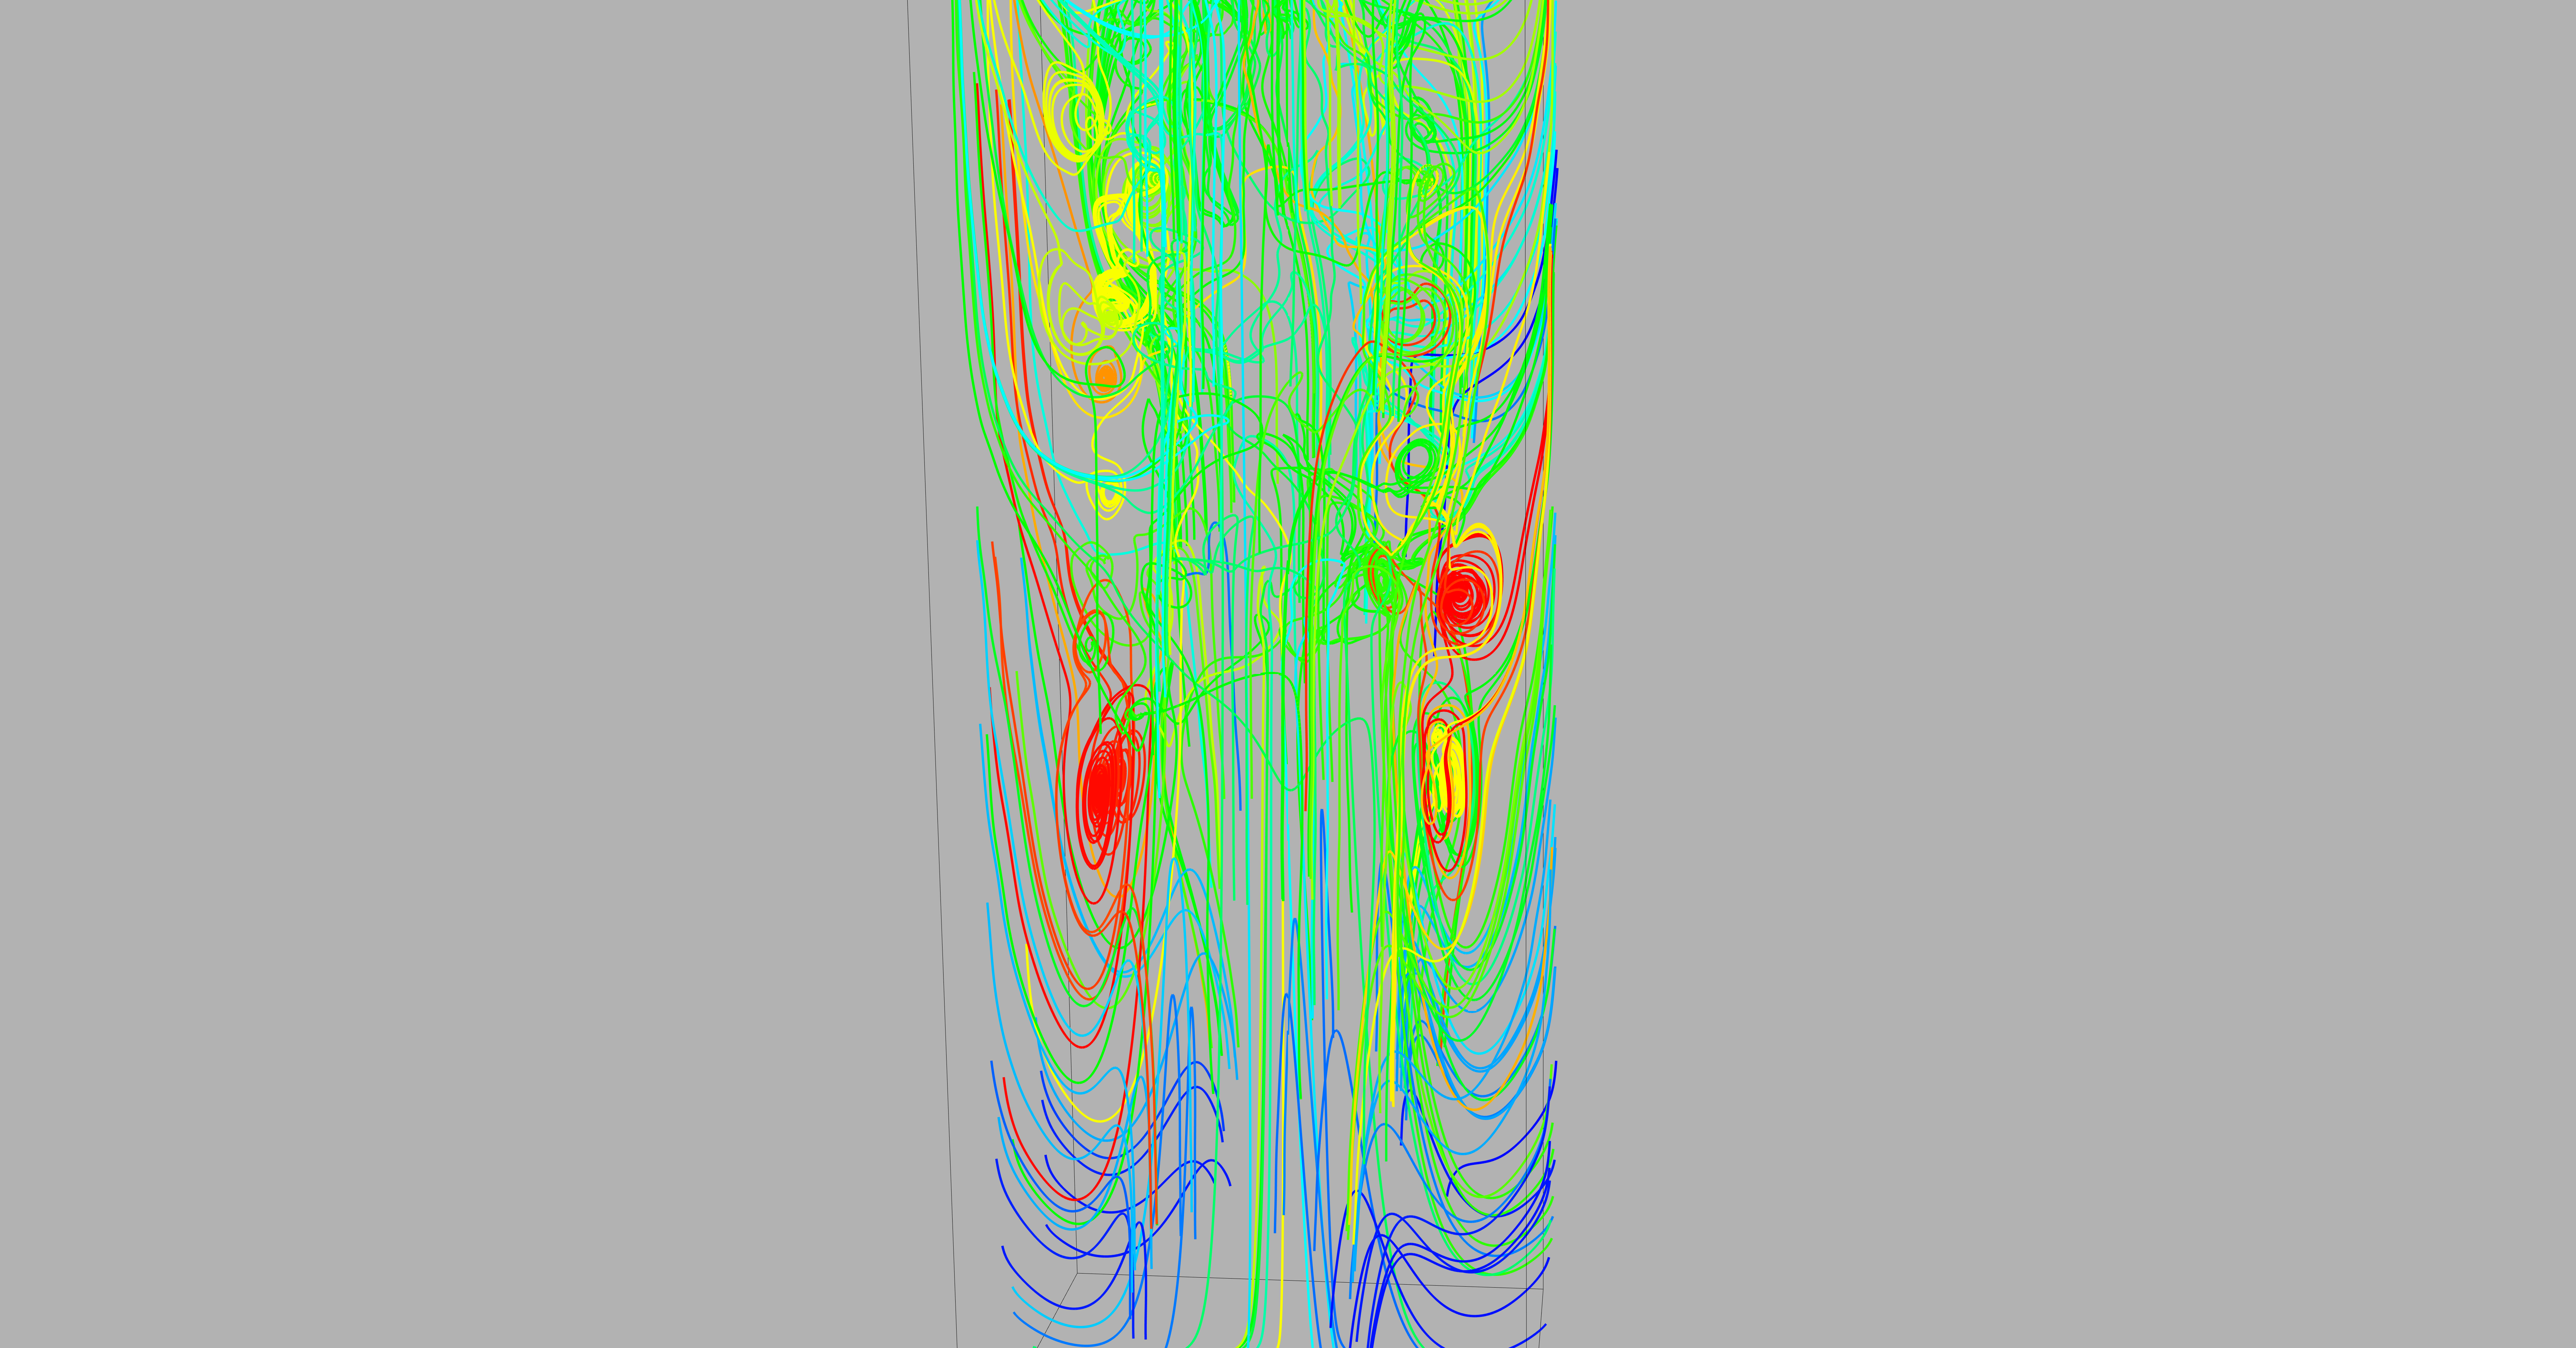
\includegraphics[height = 0.7\linewidth]{all.png}\\(a) the cluttered view of all of the streamlines in the dataset\vspace{0.2em}
		\end{minipage}
		\begin{minipage}{0.45\linewidth}
			\centering \small
			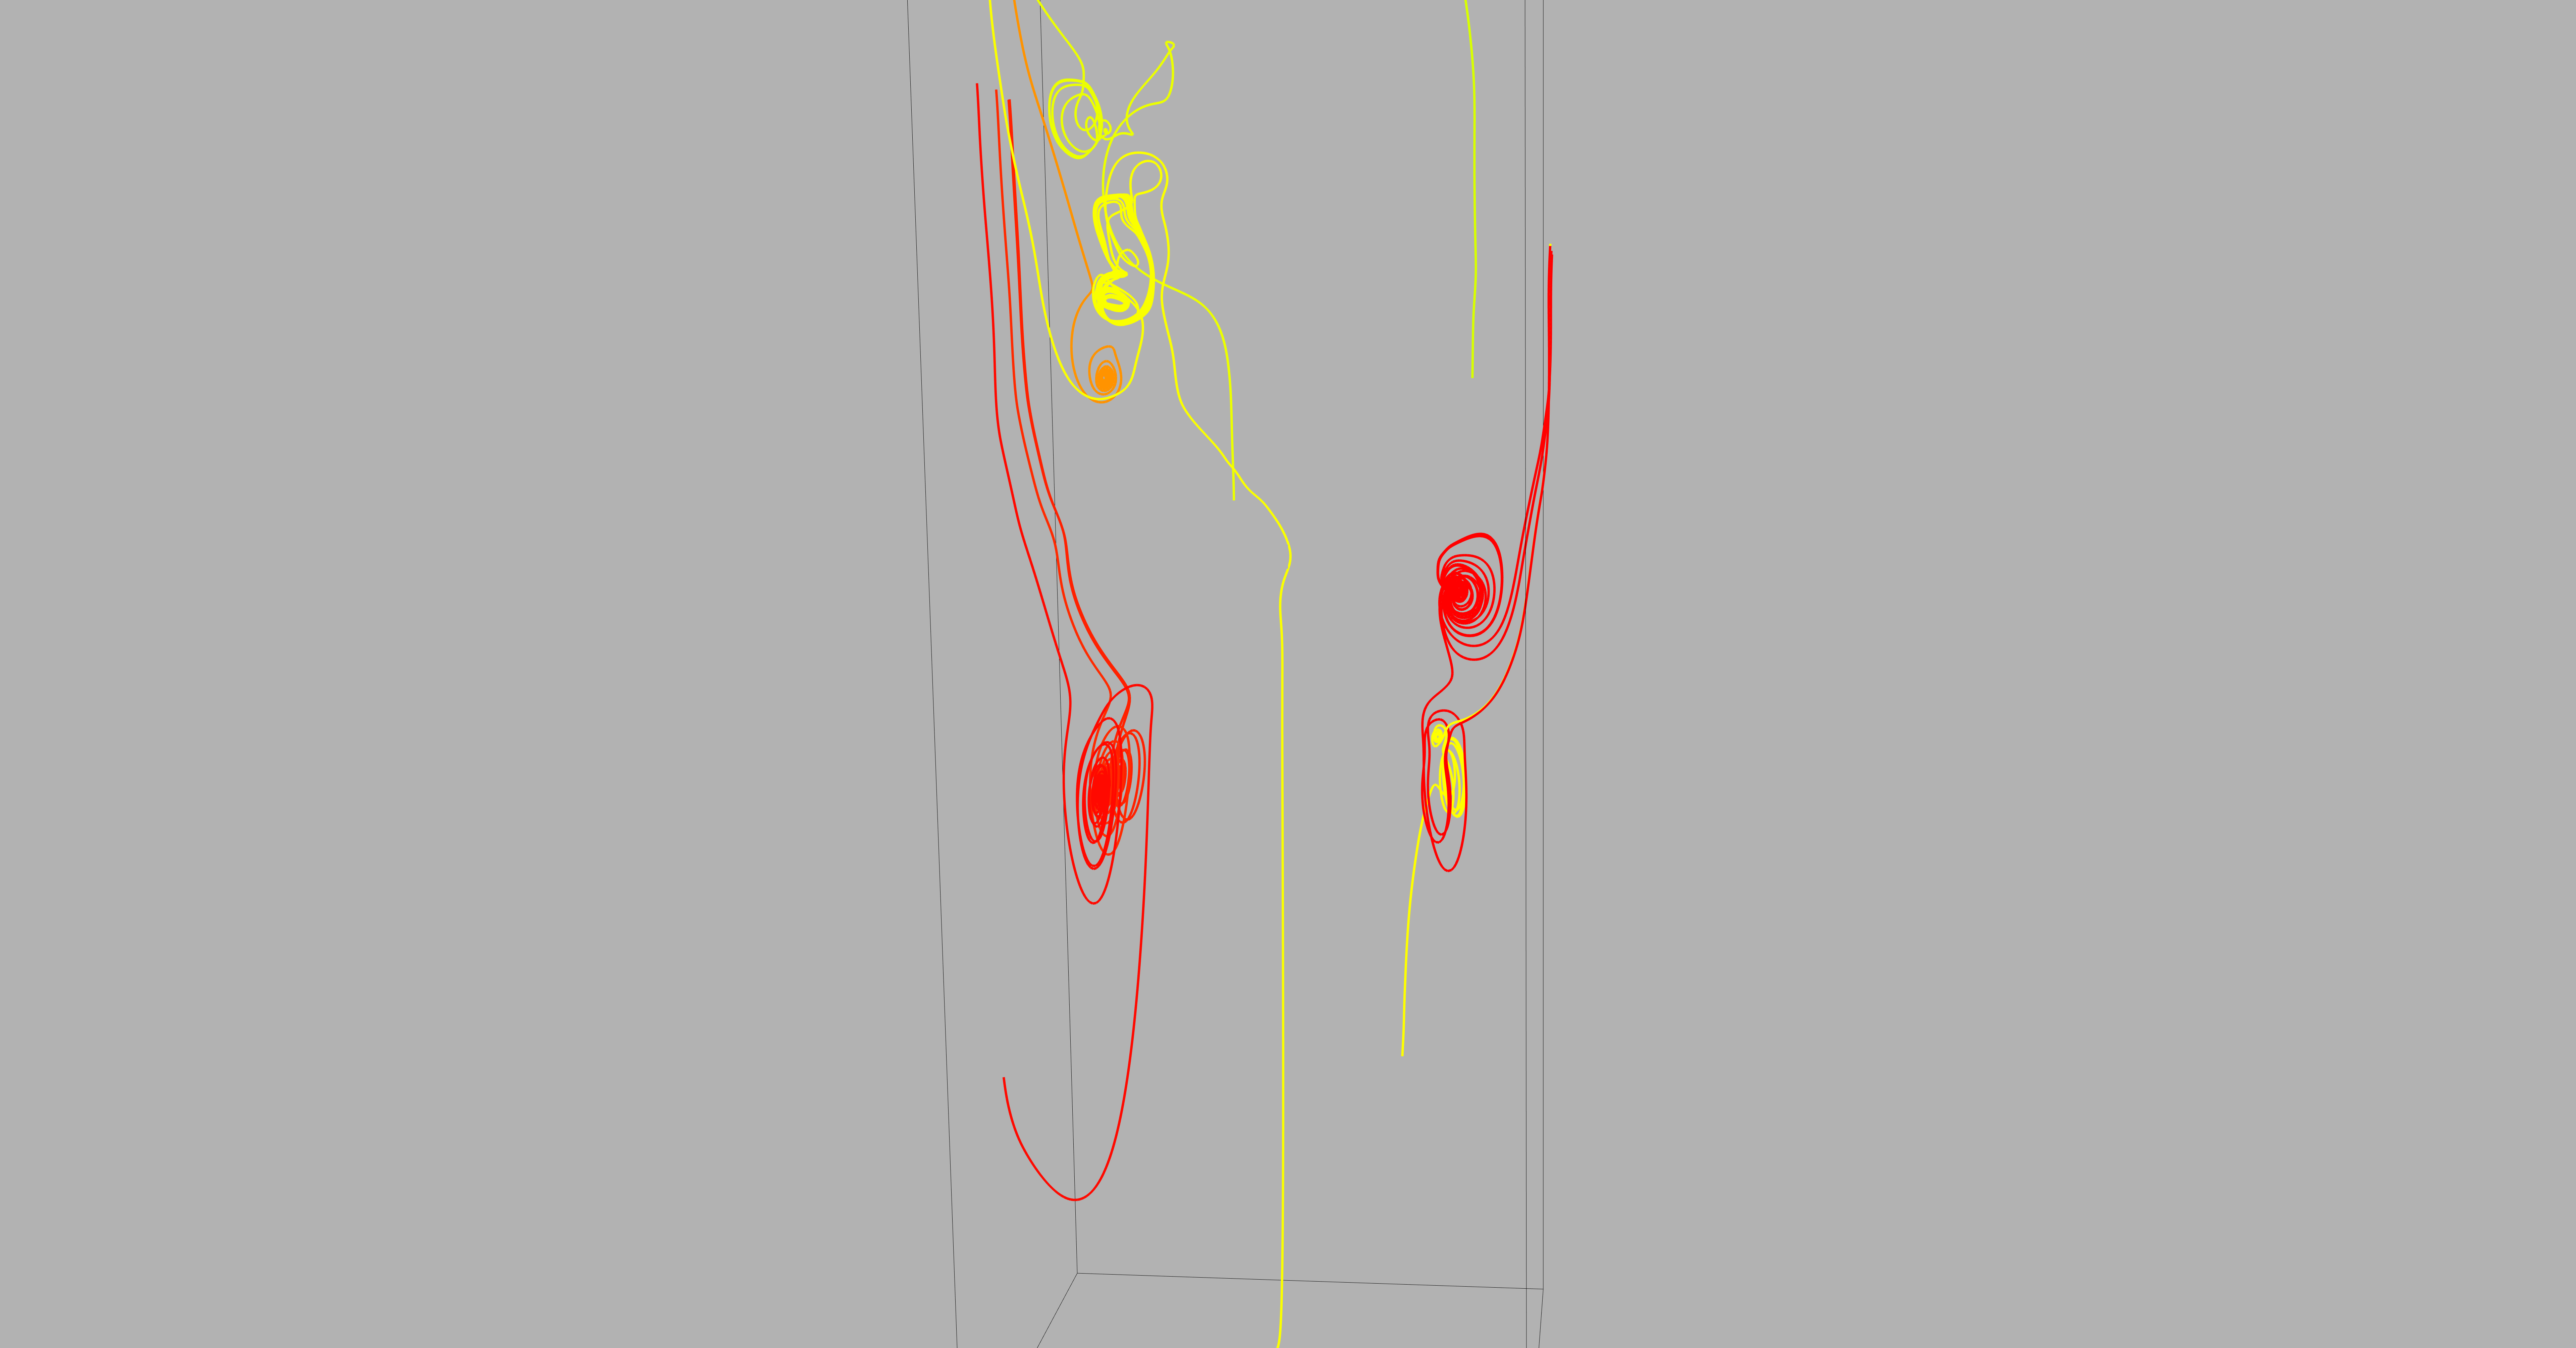
\includegraphics[height = 0.7\linewidth]{filtered.png}\\(b) the filtered streamlines above a certain complexity value \vspace{0.2em}
		\end{minipage}
	\caption{Example of the streamline filtering.}
	\label{fig:value_filter}
\end{figure}

\textbf{Local complexity maximums:}
A significant amount of clutter in the streamline display will remain if additional filtering methods are not considered.
Several streamlines in the visualization will be visually similar or provide redundant information.
We are able to only show the local maximum streamlines to filter streamlines that all represent a single region or feature of the flow.
Local maximum filtering will show streamline $v_\zeta$ only if for all of the 8 points $q$ that directly neighbor $v$ on the complexity grid, $\phi_w(v) > \phi_w(q)$.
This method allows for single streamlines representatives to be shown for each feature or region rather than several, cluttered streamlines.

\textbf{Colored plane:}
A colored plane can be used to allow the user to visualize the scalar complexity grid, $\phi_p$, directly.
A color gradient from blue to green to red is able to be defined and mapped to values in the range 0 to 3, for each of the possible box counting dimensions ratios.
Low scalar values will be displayed as blue colors, while high scalar values will be displayed as red colors.
A plane is then defined on the scalar complexity grid and each point on the plane is colored from this defined color gradient.
The user is able to control the plane through the scalar complexity grid to identfiy regions varying complexity in the grid.
Once regions of interest are identified through the color plane, the user can display streamlines near that region to understand its behavior.

\textbf{Complexity samplings}
The streamlines seeded from the region of the colored plane can be viewed in various samplings to show the different levels of complexity around the plane.
The scalar values on the colored planes are partitioned into two sets, the one-third highest scalar values and the two-thirds lowest scalar values.
Two sets of streamlines are also constructed.
For the voxels that the plane intersects, $S_{top} = \{ v_\zeta | \phi_w(v)$ is in the top one-third scalar values$\}$ and $S_{bottom} = \{ v_\zeta | \phi_w(v$) is in the bottom two-thirds scalar values $\}$.
Two values are then defined by the user to determine the percentages of $S_{top}$ and $S_{bottom}$ displayed.
An example of the plane visualizations are shown in Fig. \ref{fig:plane}.

\begin{figure}[t]
	\centering
		\begin{minipage}{0.47\linewidth}
			\centering \small
			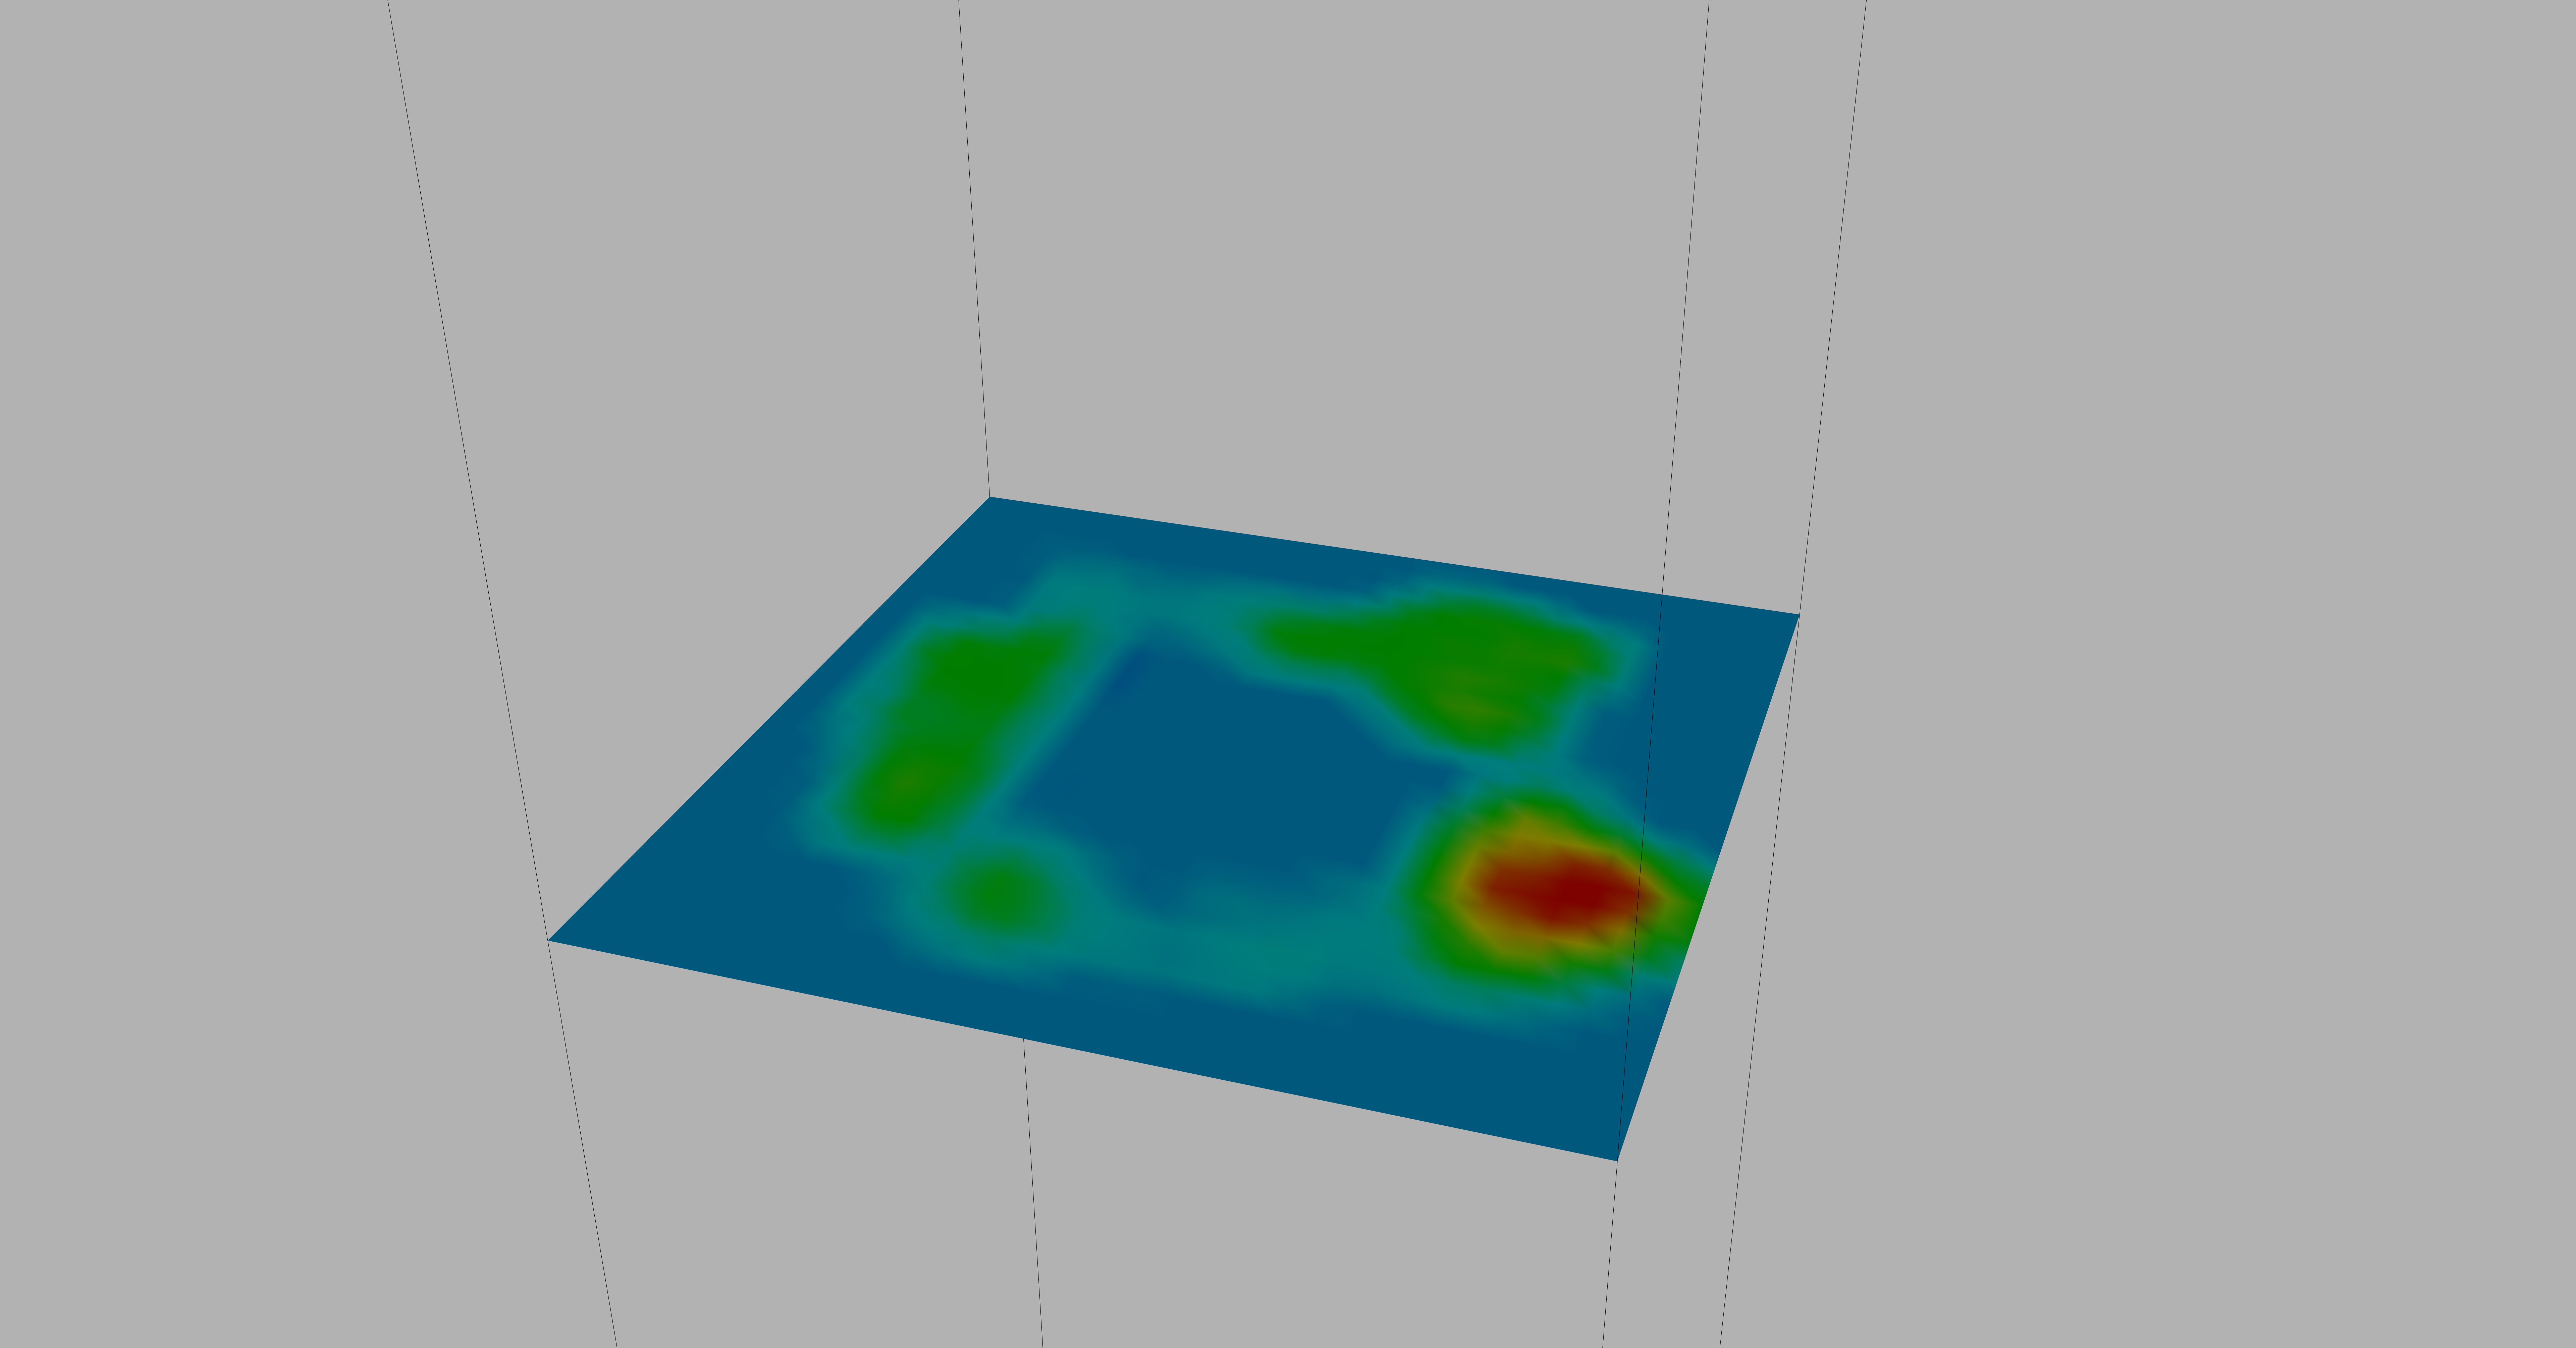
\includegraphics[height = 0.7\linewidth]{plane.png}\\(a) the plane indicating the regions of high complexity by color\vspace{0.2em}
		\end{minipage}
		\begin{minipage}{0.47\linewidth}
			\centering \small
			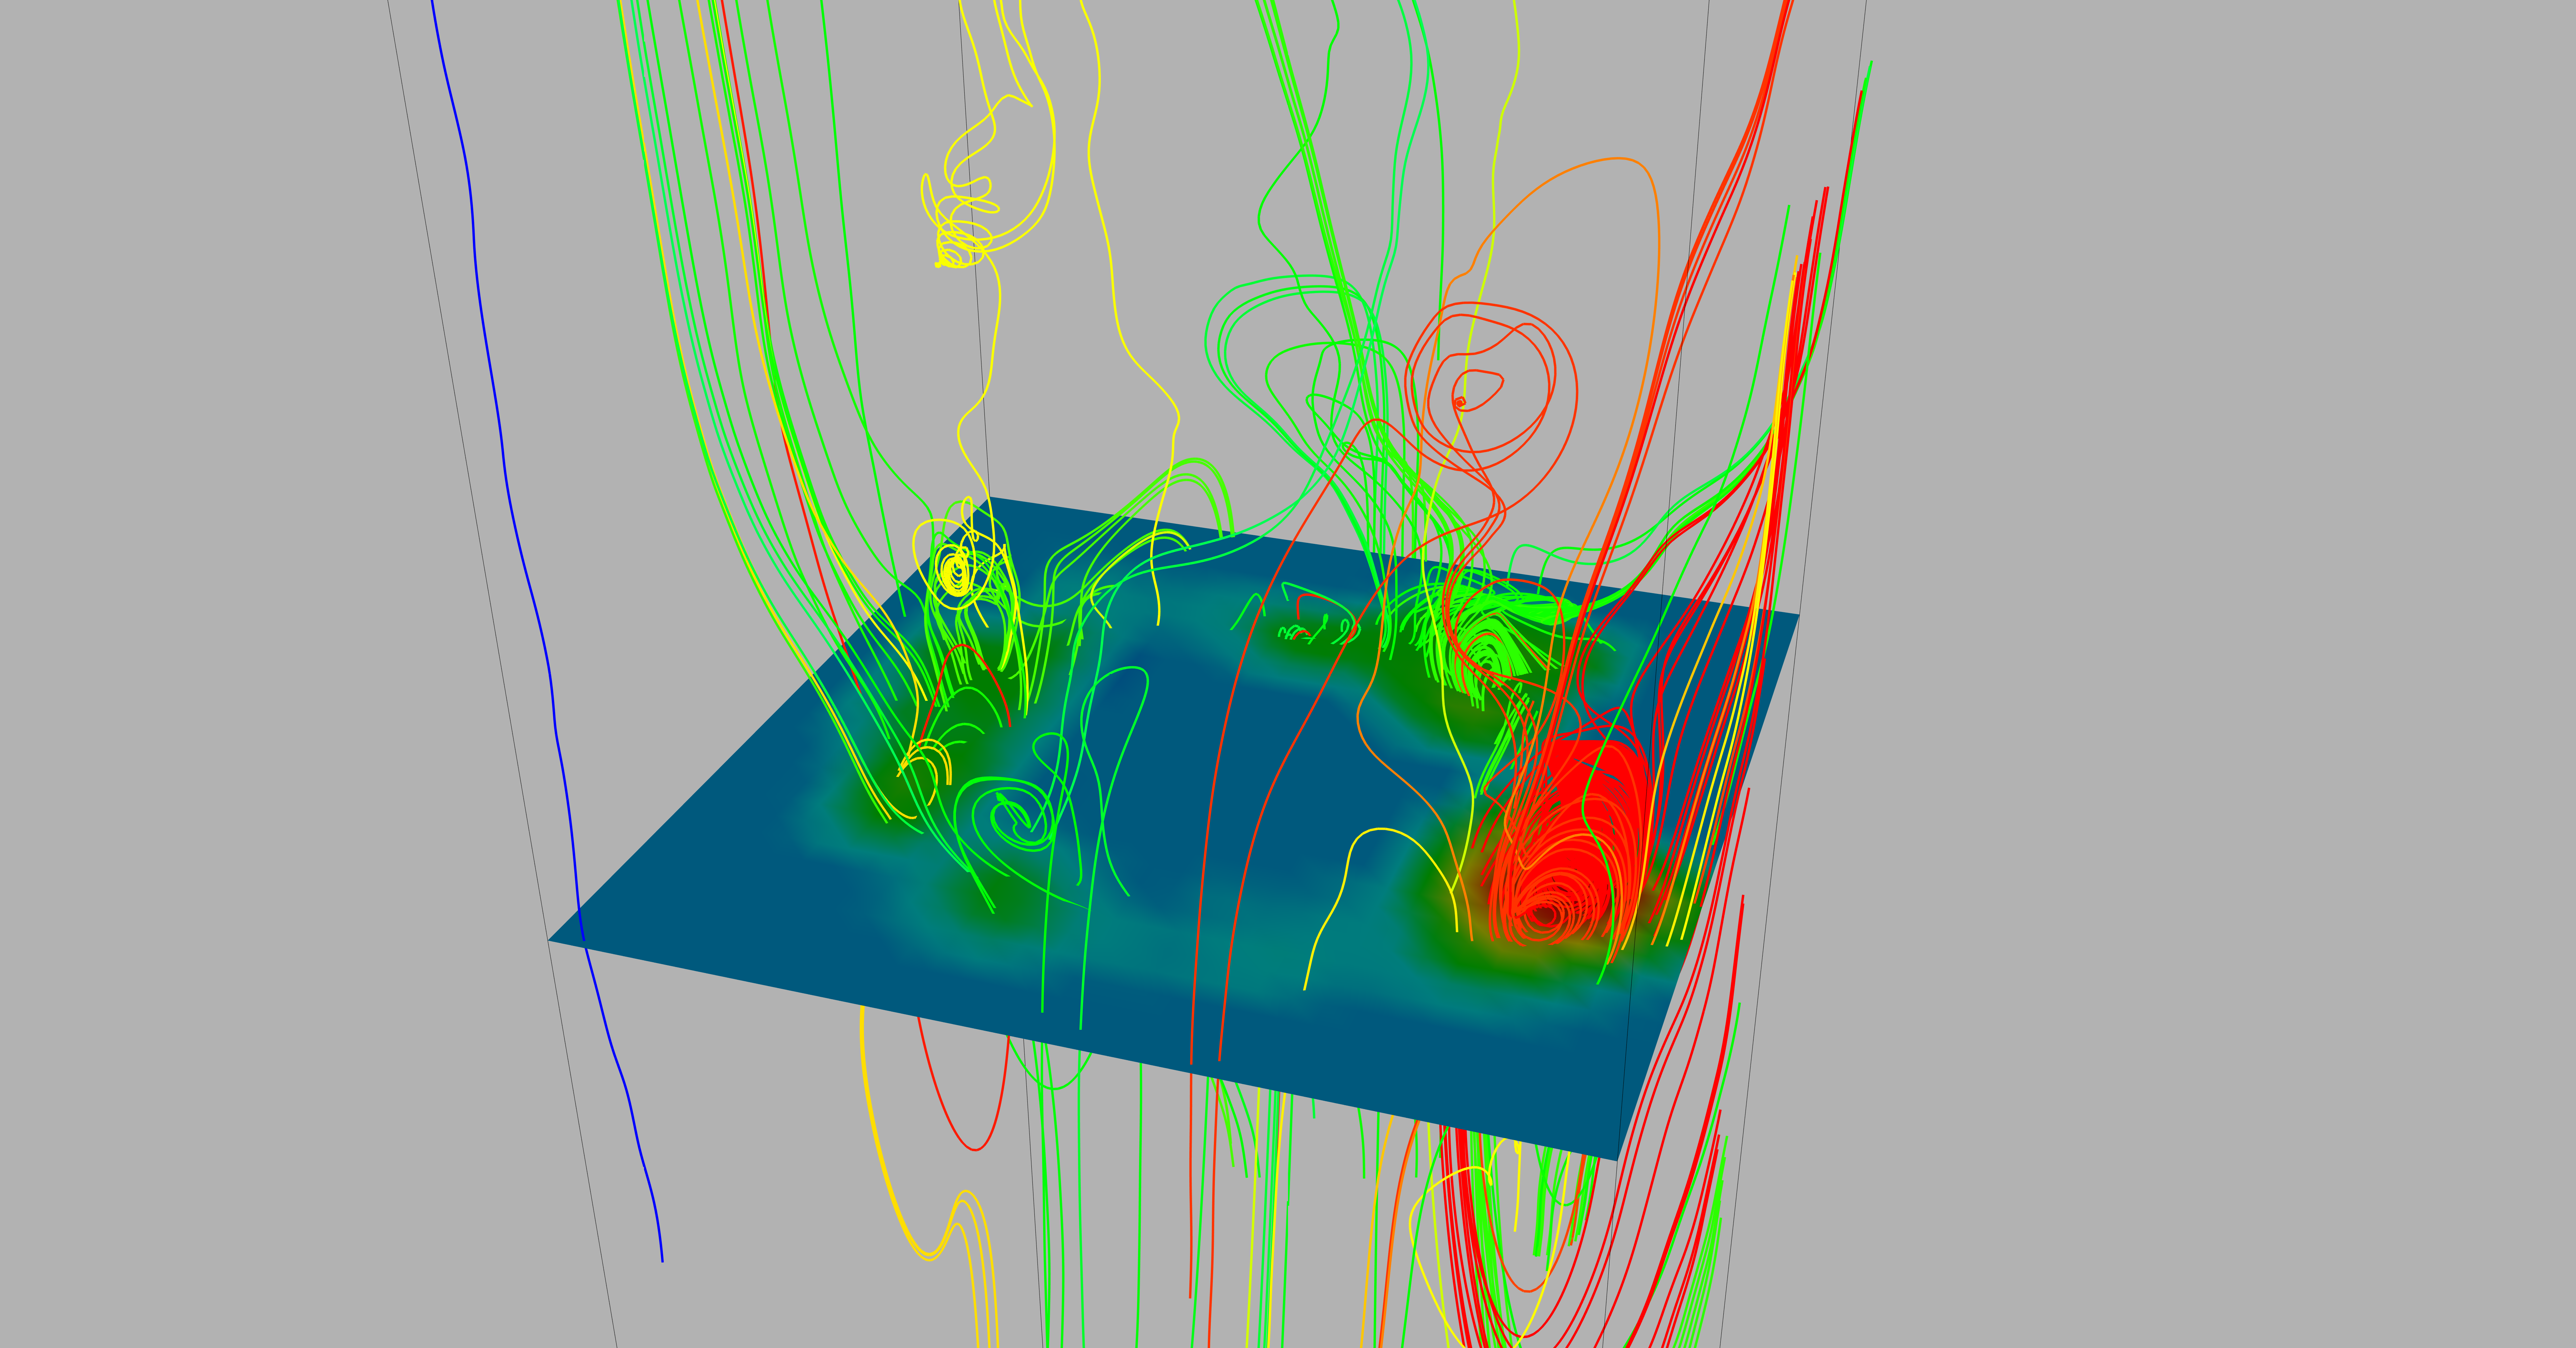
\includegraphics[height = 0.7\linewidth]{plane_line.png}\\(b) the high complexity lines near the defined plane.\vspace{0.2em}
		\end{minipage}
	\caption{Example visualizations using the colored plane.}
	\label{fig:plane}
\end{figure}

\textbf{Isosurfaces:} 
An isosurface can be used to highlight regions of the flow field with a high complexity.
An isosurface, which is defined by
\begin{equation} \{ x \mid \phi_w(x) = \sigma \}\end{equation}
where $\sigma$ is the isovalue and $\phi_w$ is the streamline complexity field, will seperate all scalar values above $\sigma$ from the values below $\sigma$ on the streamlines complexity.
This isosurface will enclose the regions of streamlines with a fractal dimension higher than the $\sigma$ value and provide a simple way to identify regions of a defined complexity.
At particularly high $\sigma$ values, the isosurface will only enclose vortices and turbulent features of the flow field that the user may have otherwise missed.

\textbf{Streamline gradient magnitudes:}
The gradient magnitudes of the streamline complexity grid can be calculated to create a new gradient magnitude scalar grid $\phi_g$.
The scalar $\phi_g(x)$ is given by $\| \nabla \phi_p(x) \|$.
Another isosurface can be used to visualization the function $\phi_g$ to identify regions of high change of turbulence or complexity.
Vortices in the flow field tend to have high complexity values recorded near their centers, with values quickly decreasing towards their boundaries.
When a high isovalue is chosen for the gradient magnitude isosurface's isovalue, the isosurface will highlight these isolated regions of turbulence or turbulent regions that quickly become smooth.
Example of isosurfaces of the scalar complexity values and gradient magnitudes are shown in Fig. \ref{fig:iso}.

\begin{figure}[t]
	\centering
		\begin{minipage}{0.47\linewidth}
			\centering \small
			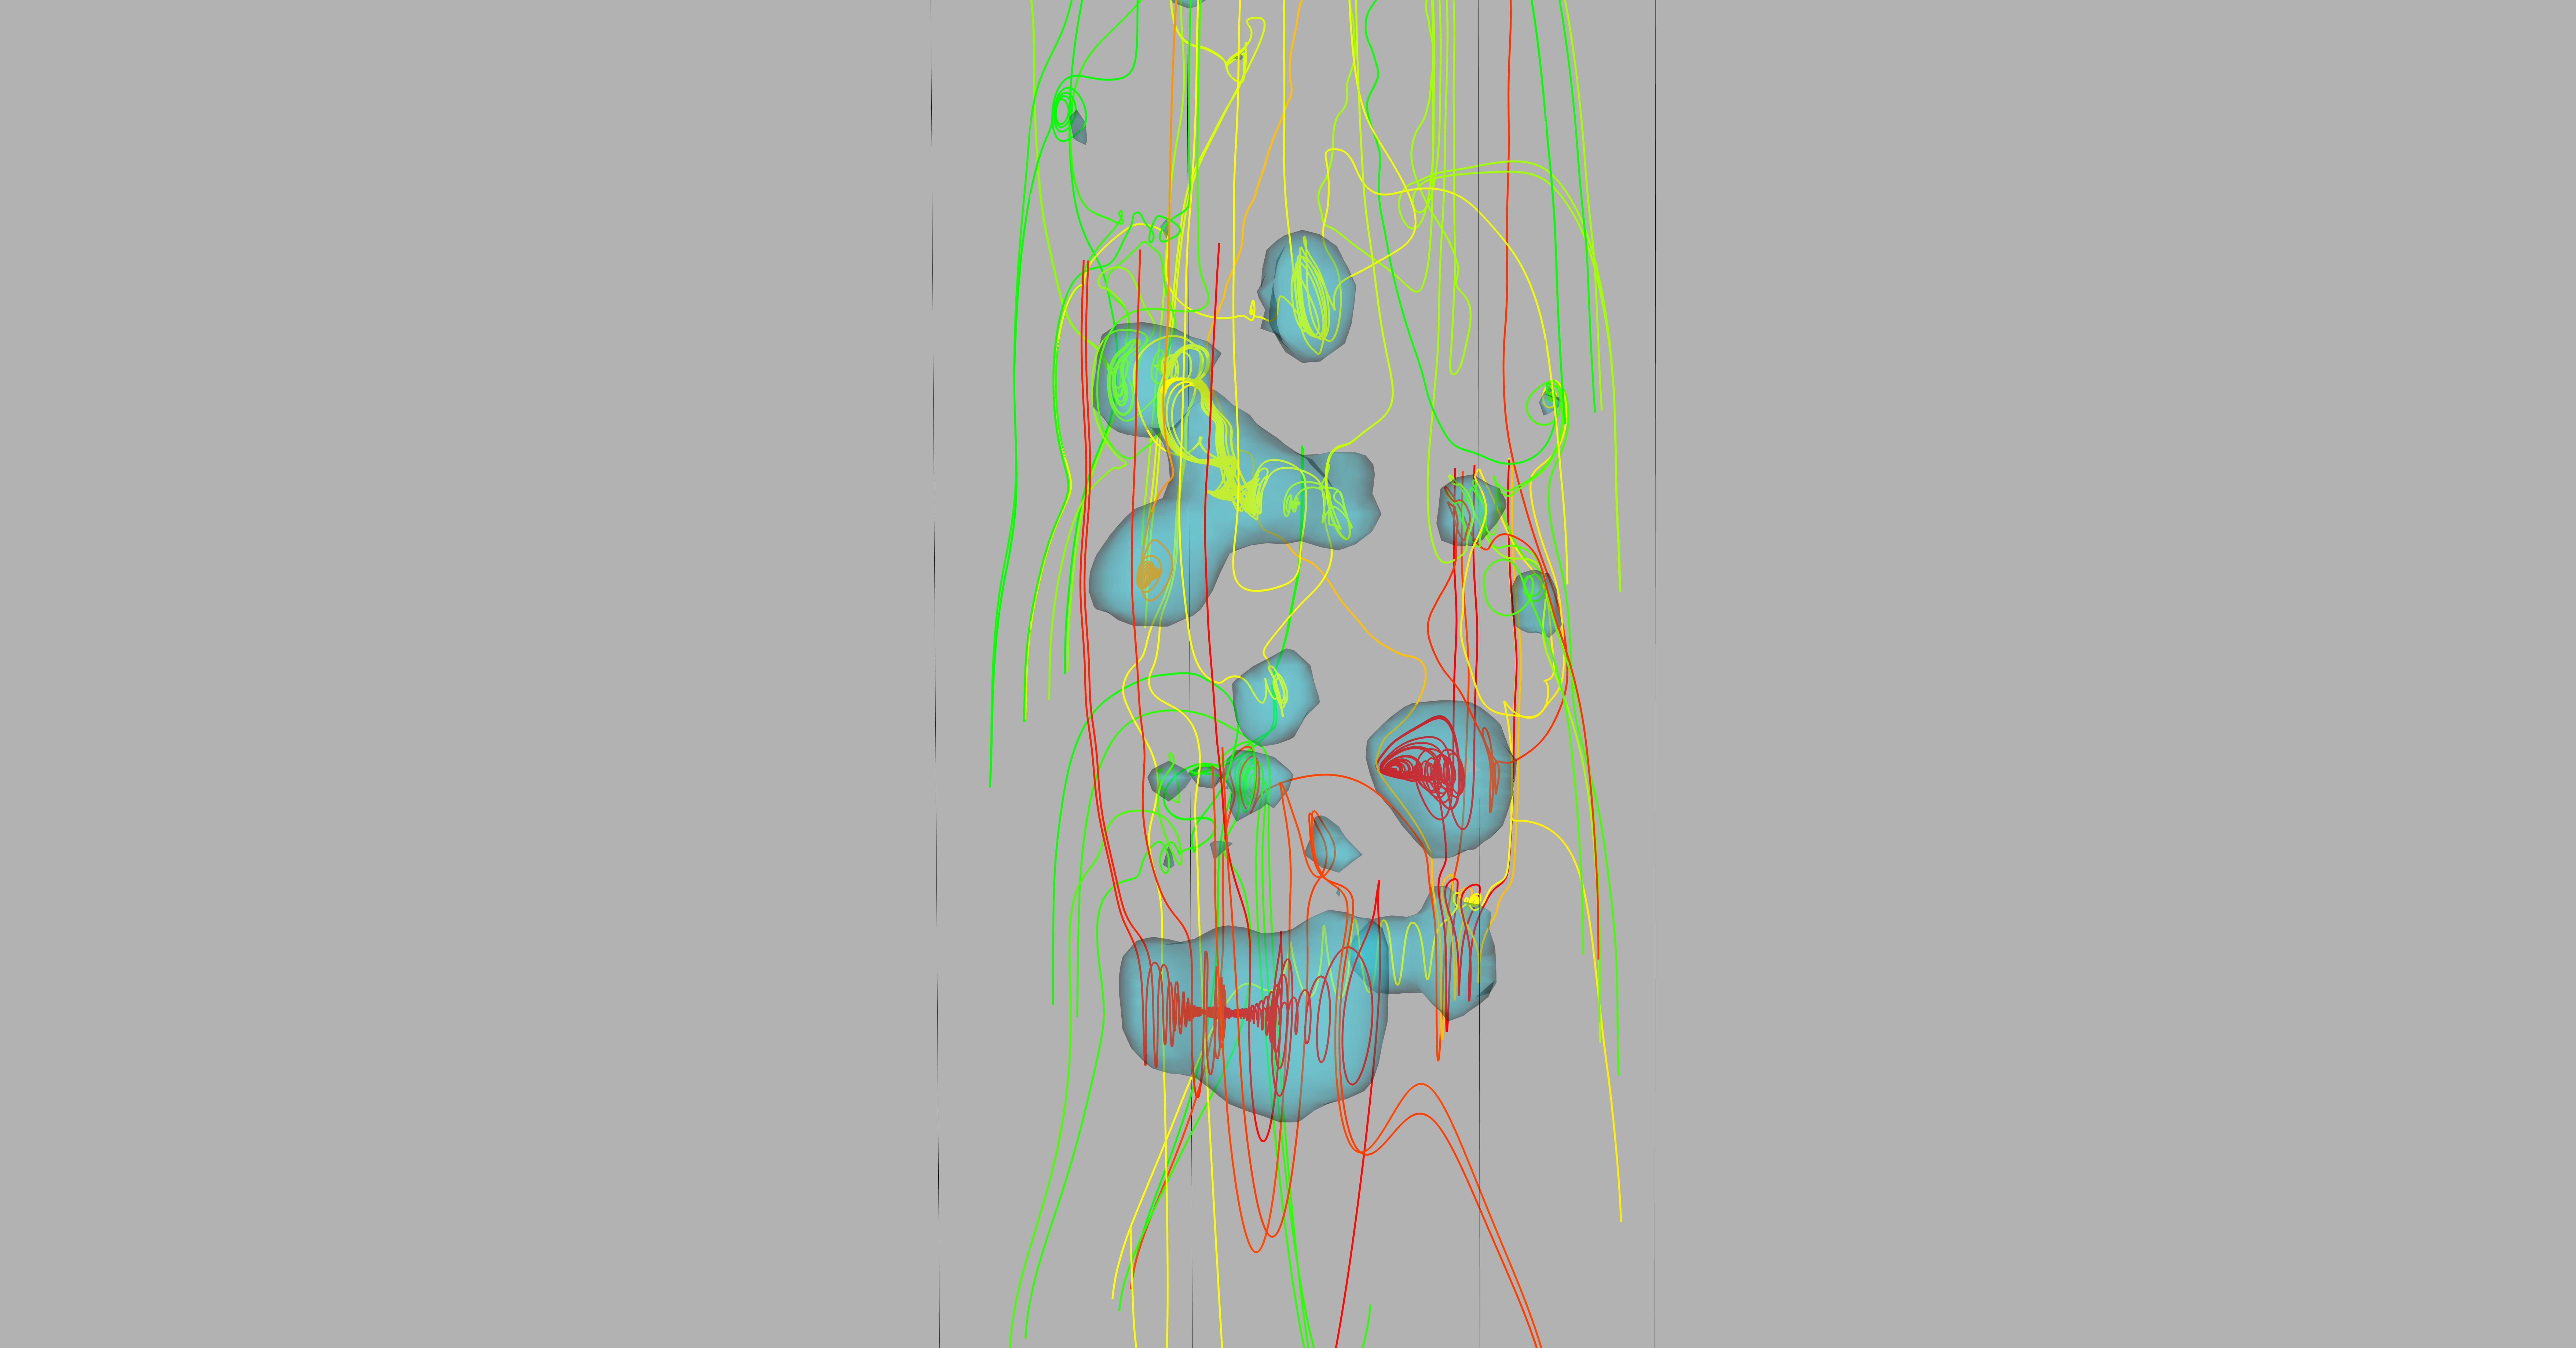
\includegraphics[height = 0.7\linewidth]{iso.png}\\(a) the scalar value isosurface enclosing high complexity regions\vspace{0.2em}
		\end{minipage}
		\begin{minipage}{0.47\linewidth}
			\centering \small
			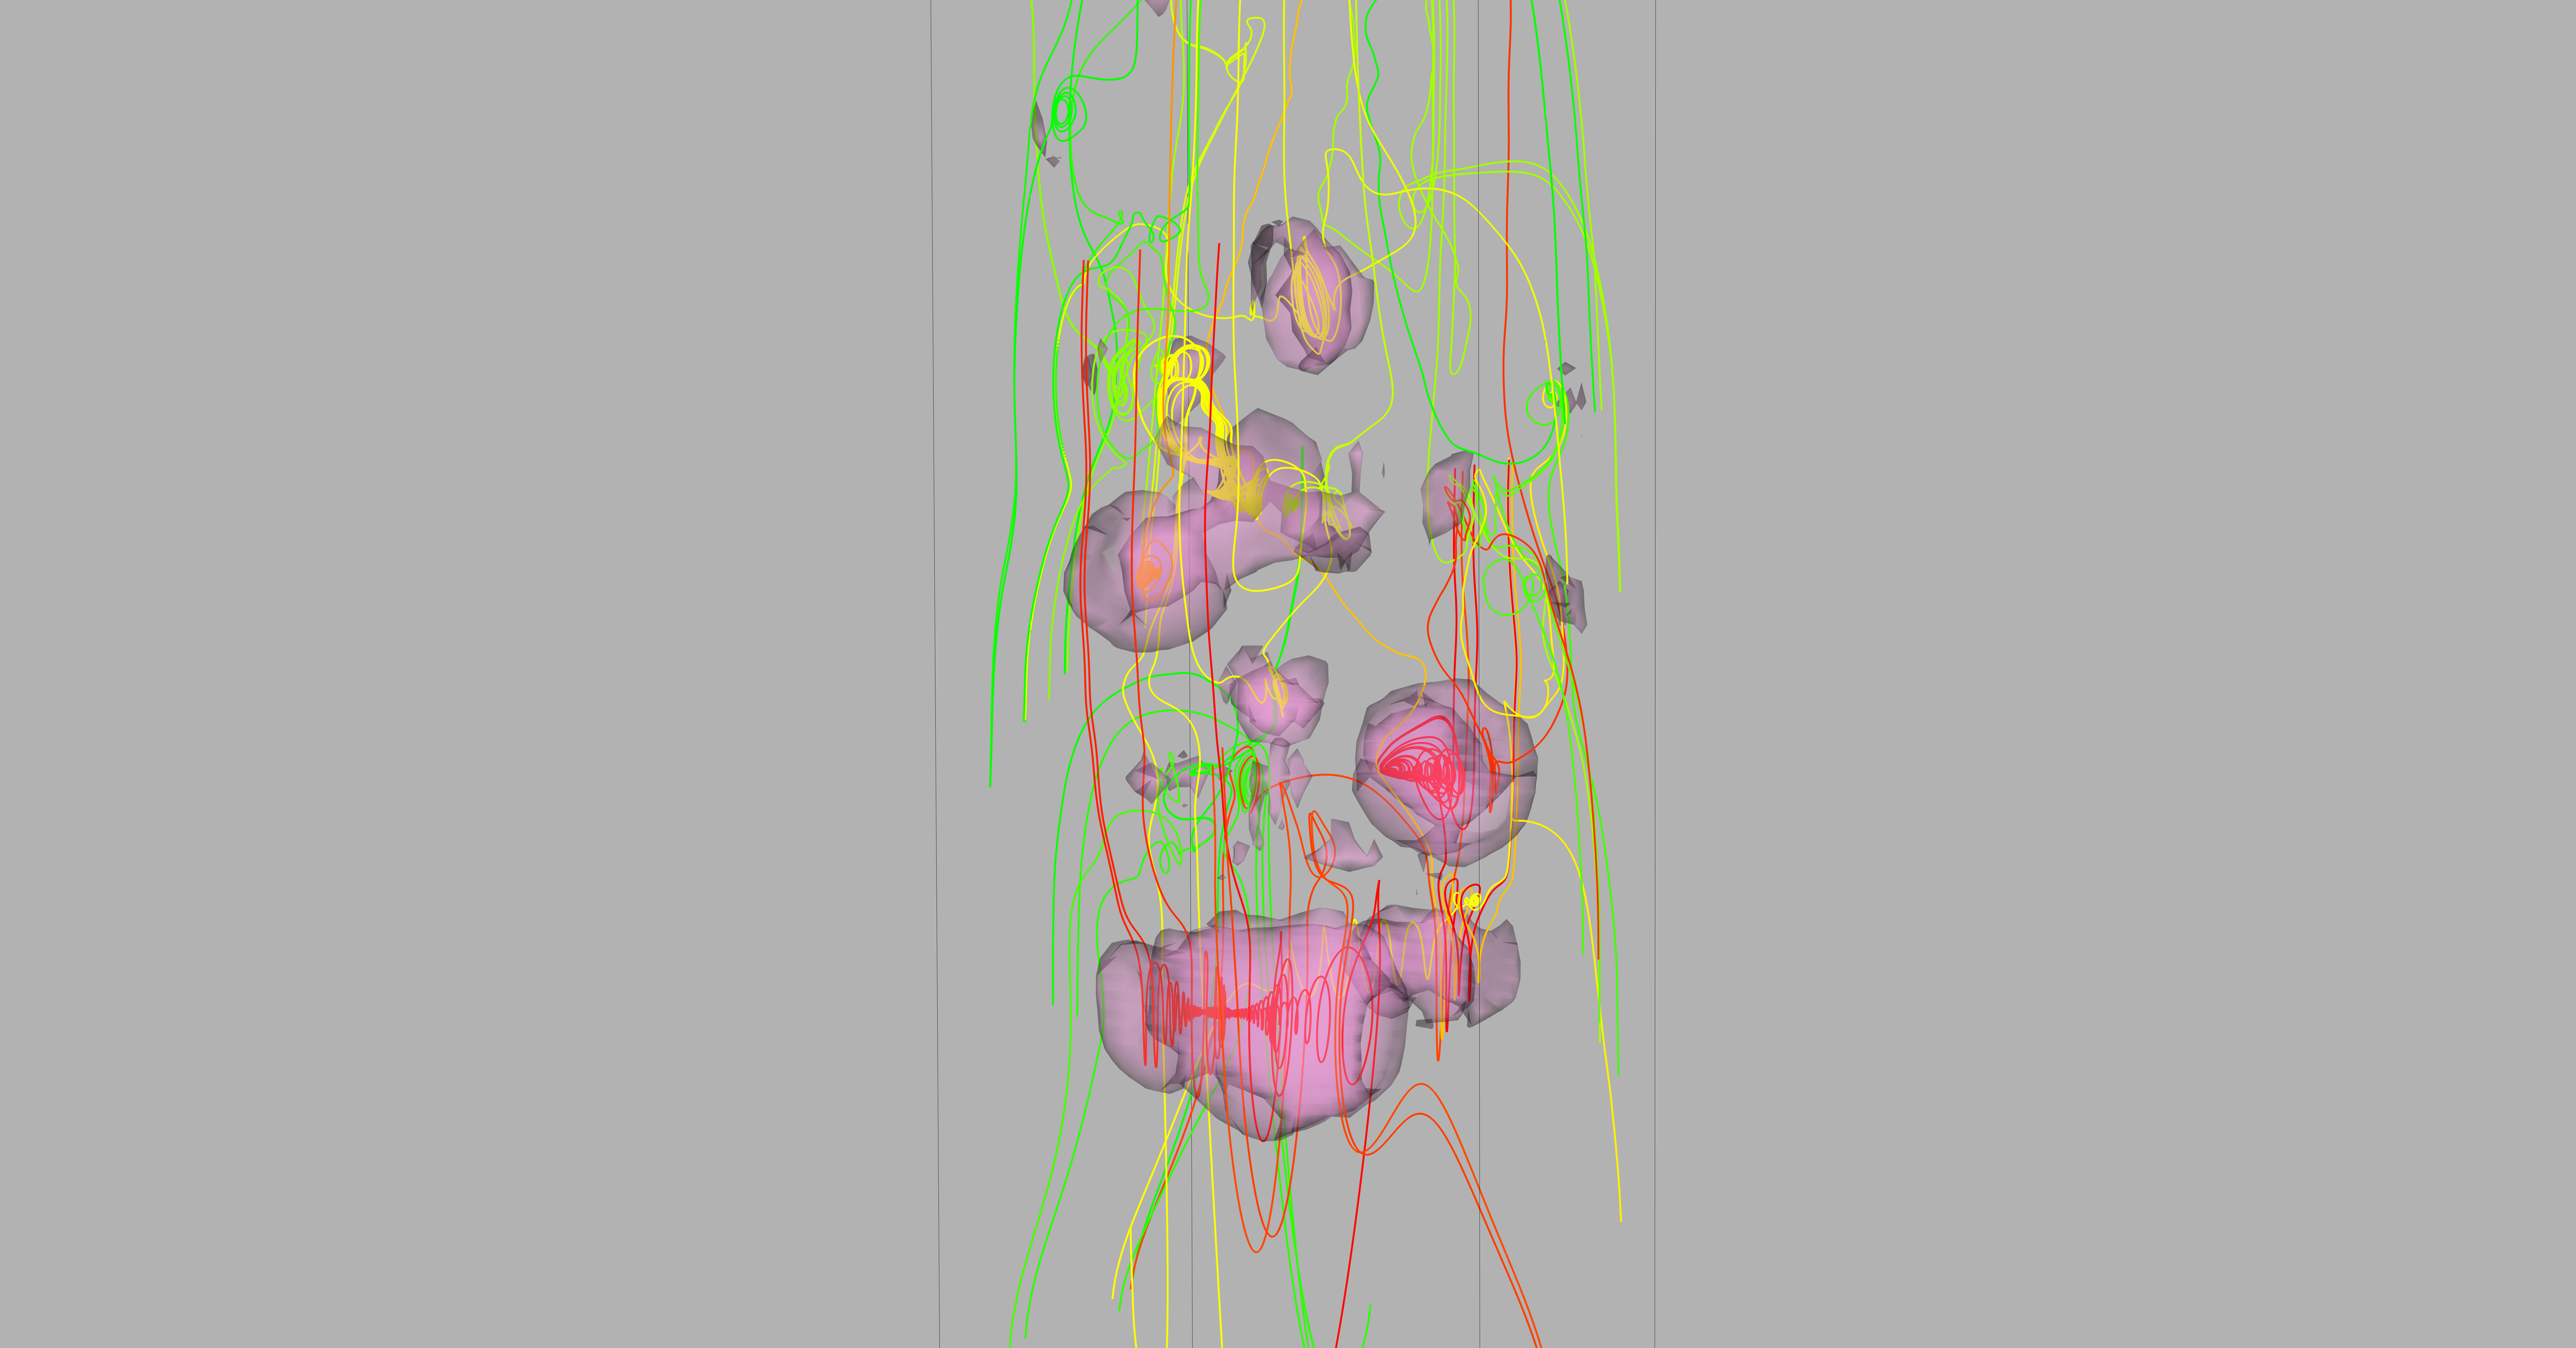
\includegraphics[height = 0.7\linewidth]{grad.png}\\(b) the gradient isosurface enclosing regions of high complexity change. \vspace{0.2em}
		\end{minipage}
	\caption{Example visualizations using the colored plane.}
	\label{fig:iso}
\end{figure}

\section{Examples}

\section{Evaluation}

\section{Summary and Future Work}

\end{document}
